\documentclass[11pt,a4paper]{article}

\usepackage[utf8]{inputenc}
\usepackage[T1]{fontenc}
\usepackage{amsmath,amssymb,amsthm}
\usepackage{mathtools}
\usepackage{graphicx}
\usepackage{booktabs}
\usepackage{hyperref}
\usepackage[margin=1in]{geometry}
\usepackage{authblk}
\usepackage{caption}
\usepackage{longtable}

\hypersetup{colorlinks=true,linkcolor=black,citecolor=black,urlcolor=blue}

\newtheorem{theorem}{Theorem}
\newtheorem{proposition}[theorem]{Proposition}
\newtheorem{definition}[theorem]{Definition}

\newcommand{\Ztwo}{\mathbb{Z}_2}
\newcommand{\Qsix}{Q_6}
\newcommand{\xor}{\oplus}

\title{A machine-checked formalization of the Fuxi hexagram system:
group structure, divination-induced Markov dynamics,
and corrections to the received analysis}

\author{Muning An\thanks{Correspondence: \texttt{everest9812@gmail.com}}}
% Pinned rather than \today so that a rebuild reproduces the committed PDF.
\date{22 July 2026}

\begin{document}

\maketitle

\begin{abstract}
The Fuxi Earlier Heaven arrangement of the sixty-four hexagrams has been read as
a binary system since Leibniz, and a series of algebraic and coding-theoretic
studies have since described parts of its structure. Those descriptions are
stated informally, and their quantitative claims have not been checked against a
running model. We give a complete computational formalization of the system and
an open-source suite that machine-checks every quantitative claim it makes. We
first fix a bottom-up bit encoding and show by exhaustion that the recursive
doubling generation produces the full set of six-bit strings under either of the
two line-placement conventions in circulation. We then prove that the
changing-line mechanism is bitwise exclusive-or with a mutation mask, and
identify the resulting transition structure as the elementary abelian group
$\Ztwo^6$, whose Cayley graph is the six-dimensional hypercube. Extending the
model to a Markov chain exposes a discrepancy that informal treatment had
hidden. Under the yarrow-stalk procedure a yang line changes with probability
$3/8$ and a yin line with probability $1/8$, so the mutation mask is not
independent of the current state even though its marginal rate is $1/4$. The
kernel the procedure actually induces is therefore asymmetric, and its
stationary distribution is not uniform but the product form
$\pi(h) \propto (3/4)^{\text{yin}}(1/4)^{\text{yang}}$, which places $729$ times
more mass on the all-yin hexagram than on the all-yang hexagram. Turning to the
arrangements themselves, we confirm that the King Wen sequence is built from
thirty-two couplets related by inversion, or by complementation where a hexagram
is its own inversion, and we count the improbability of that structure exactly
at $8.9 \times 10^{-45}$ under a random ordering. The same sequence is
unremarkable as a code, sitting two standard deviations above a random null on
consecutive distance, so its two possible organizing criteria come apart. Of
forty-seven checked claims, twenty-five are confirmed, five are refined, nine
are new, and eight are corrected. The corrections include a clustering
coefficient reported as $5/12$ that is exactly zero because the state graph is
bipartite, a mutual information of $1.132$ bits that is $1.233$ bits once the
state dependence is carried through, a genetic-code dimension count that
overstates the independent binary degrees of freedom by a factor of two per
nucleotide, and the bit-weight convention under which the Earlier Heaven
arrangement is binary counting. The results are reproducible from a single
command, and we state explicitly which conclusions are formal theorems, which
are exhaustive machine checks, and which are estimates under a stated model of
how the divining pile is divided.
\end{abstract}

\noindent\textbf{Keywords:} Fuxi hexagram arrangement; binary encoding;
elementary abelian group; hypercube; Markov chain; yarrow-stalk divination;
reproducible verification

\section{Introduction}

The sixty-four hexagrams of the \emph{Yijing} are six-line figures built from two
kinds of line. In 1703 Leibniz published an account of binary arithmetic that
explicitly connected his notation to hexagram diagrams sent from China by the
Jesuit Joachim Bouvet~\cite{aiton1981gorai}. The correspondence between the two
line types and the digits $0$ and $1$ has been revisited many times since, and
the Fuxi Earlier Heaven arrangement in particular has been analysed as an
algebraic object~\cite{goldenberg1975algebra,schoter1998boolean,schoter2008bipolar}
and as a code~\cite{hayata2012coding}.

These treatments share a methodological gap. They are stated as prose and
hand-derived arithmetic, and their numerical claims have not been executed. That
is a problem for two reasons. First, several of the quantities involved are easy
to state and hard to compute by inspection, including graph invariants of a
$64$-vertex graph and entropies of a joint distribution over four line states.
Second, the system carries a long interpretive tradition, which makes it
unusually easy for a claim to be repeated because it sounds structurally
plausible rather than because it has been checked.

The practical consequence is that the received description of the system
contains errors that survive precisely because nobody has run it. A clustering
coefficient is reported for the state-transition graph, and the graph in
question is bipartite and therefore has none. A Markov chain is derived from the
yarrow-stalk divination procedure under an independence assumption that the
procedure does not satisfy. A count of binary degrees of freedom in the genetic
code is used to reach the number $64$ by a route that would in fact give $512$.

This paper closes that gap. We give a formalization that is complete enough to
execute, and an accompanying suite that checks every quantitative claim the
formalization makes. Our contributions are the following.

\begin{enumerate}
\item We fix a bottom-up bit encoding and show by exhaustive construction that
the recursive doubling generation attributed to Shao Yong yields exactly the set
of six-bit strings, under either of the two conventions for where a new line is
placed. This separates the part of the binary reading that is
convention-independent, namely the set, from the part that is not, namely the
sequence (Sections~\ref{sec:encoding} and~\ref{sec:orderings}).

\item We prove that the changing-line mechanism is bitwise exclusive-or with a
mutation mask, and verify the proof on all $4^6$ assignments of the four
traditional line states. We then identify the transition structure as the
elementary abelian group $\Ztwo^6$. The three algebraic properties that earlier
treatments list separately are the group axioms, and the state graph is the
Cayley graph of that group (Section~\ref{sec:automaton}).

\item We model the yarrow-stalk procedure exactly and show that it induces a
transition kernel different from the one usually assumed. A yang line changes
three times as often as a yin line, so the mutation mask is state dependent. The
induced kernel is asymmetric and its stationary distribution is not uniform
(Sections~\ref{sec:yarrow} and~\ref{sec:kernels}).

\item We compute the topological and information-theoretic quantities directly
from the model rather than from quoted formulas, and report where the computed
values differ from the received ones (Section~\ref{sec:results}).

\item We turn the model on the arrangements themselves. The couplet structure
tradition ascribes to the King Wen sequence holds exactly, and we count its
improbability under a random ordering rather than estimating it. The same
sequence turns out not to be optimized as a code, so the symmetry and distance
criteria come apart (Section~\ref{sec:orderings}).

\item We release the verification suite. Every number in this paper is produced
by a single command, and each check records whether it confirms, refines,
corrects, or adds to the prior account (Section~\ref{sec:suite}).
\end{enumerate}

We are deliberately narrow about what these results mean. The system is a
six-bit finite state machine. Nothing here bears on the interpretive or
divinatory tradition, and nothing here supports the claim that the arrangement
anticipated any later scientific development. Section~\ref{sec:scope} states the
boundary explicitly, because the surrounding literature does not always do so.

\section{Related work}

\paragraph{Historical and philological readings.}
The transmission of the diagrams to Leibniz through Bouvet, and the subsequent
reconstruction of that exchange, are documented by Aiton and
Shimao~\cite{aiton1981gorai}. A recurring question is whether the binary reading
is intrinsic to the arrangement or projected onto it, since Leibniz assigned the
highest bit weight to the bottom line and later authors have not. Maitre argues
that the binary structure follows from the generation method itself and is
therefore not an artifact of reading direction~\cite{maitre2023fuxi}. That
argument is about the diagram; it does not supply an executable model, and it
leaves the enumeration order unaddressed. We verify the set-level claim and
extend it to the ordering in Section~\ref{sec:encoding}.

\paragraph{Algebraic treatments.}
Goldenberg analysed hexagram transformations group-theoretically and reported a
non-abelian structure~\cite{goldenberg1975algebra}. Sch\"oter developed a
Boolean-algebra framework covering correspondence and bipolar
change~\cite{schoter1998boolean,schoter2008bipolar}. These works operate on the
same underlying set as we do, and the difference is which group action is in
view. Two distinct groups act on the sixty-four hexagrams. Permuting the six
line positions gives $S_6$, which is non-abelian. Flipping line values gives the
elementary abelian group $\Ztwo^6$. The changing-line mechanism lives entirely
in the second, which is why the structure we describe in
Section~\ref{sec:automaton} is abelian and is not in conflict with a non-abelian
result about a different action. We make the separation explicit and compute the
order of the group the two generate together.

\paragraph{Coding-theoretic treatments.}
Hayata computed Hamming distances between consecutive hexagrams under several
orderings and mapped the hexagrams onto a six-dimensional
hypercube~\cite{hayata2012coding}. That work establishes the hypercube
embedding, which we take as given, and it reports distance statistics rather
than graph invariants. The clustering coefficient we correct in
Section~\ref{sec:topology} is therefore not a claim of that paper. It is a value
carried in the informal restatement of the system that this work formalizes, and
we have not traced it to a primary source.

\paragraph{Structure of the King Wen sequence.}
That the King Wen sequence pairs its hexagrams by inversion, with complementation
substituted for the eight hexagrams that inversion leaves fixed, is long
established and widely repeated. What has not accompanied it is a quantitative
statement of how much structure that represents. We verify the claim
exhaustively and, more usefully, count its improbability under a random ordering
exactly rather than estimating it, which turns a qualitative observation into a
number (Section~\ref{sec:orderings}).

\paragraph{Probabilistic models of the divination procedure.}
The line-state probabilities of the yarrow-stalk method have been derived
combinatorially and checked by
simulation~\cite{sun2018dayan,tang2017monte}. Those studies compute the
marginal distribution over the four line states, which is what the procedure
directly produces. They do not ask what transition kernel the procedure induces
on the space of hexagrams. That question is where the independence assumption
enters, and it is where we find the discrepancy reported in
Section~\ref{sec:kernels}.

\paragraph{Structural comparisons with the genetic code.}
Both the hexagram set and the codon set have $64$ elements, and this has
motivated a body of comparative
work~\cite{hu2017iching,castrochavez2012defragged,lien1997physicochemical}. The
comparisons rest on a count of binary dimensions per nucleotide. We show in
Section~\ref{sec:genetic} that the three dichotomies usually cited are not
independent, which changes the count although it does not change the conclusion
that both sets have $64$ elements.

\section{Formal model}
\label{sec:model}

\subsection{Encoding and the doubling method}
\label{sec:encoding}

A hexagram is six stacked lines, each either yang or yin. Traditional line names
run from the bottom upward. We write a hexagram as a tuple
$(b_1,\dots,b_6) \in \{0,1\}^6$ with $b_1$ the bottom line, and set $b_i = 1$ for
yang and $b_i = 0$ for yin.

We adopt the bottom-up bit-weight convention, in which the bottom line is the
least significant bit:
\begin{equation}
V(h) \;=\; \sum_{i=1}^{6} b_i \, 2^{\,i-1}.
\label{eq:encoding}
\end{equation}
Under Equation~\eqref{eq:encoding} the all-yin hexagram Kun is $0$ and the
all-yang hexagram Qian is $63$, and $V$ is a bijection onto $\{0,\dots,63\}$.

The recursive doubling generation attributed to Shao Yong starts from a single
undifferentiated symbol and splits every symbol in two at each step. Writing
$G(n)$ for the set of $n$-line symbols, $G(0)$ is a singleton and each step
replaces every symbol by two symbols differing in one new line.

\begin{theorem}
\label{thm:doubling}
$|G(n)| = 2^n$, and $G(6)$ is the full set of six-bit strings.
\end{theorem}

\begin{proof}
By induction. $|G(0)| = 1 = 2^0$. Each element of $G(k)$ produces exactly two
elements of $G(k+1)$, and the two are distinguished by the value of the new
line, so the branches are disjoint and $|G(k+1)| = 2|G(k)|$. Since the
construction never identifies two distinct symbols, $G(n)$ injects into
$\{0,1\}^n$, and equality of cardinalities gives surjectivity.
\end{proof}

Theorem~\ref{thm:doubling} is convention-independent in a sense worth making
precise, because the placement of the new line is exactly the point on which
readings differ. The new line may be added above the existing ones, becoming the
new most significant bit, or below them, shifting the existing lines up. We
verify in Section~\ref{sec:results} that both placements generate the same set
and, with the natural enumeration at each level, the same order.

The set carries a Boolean lattice structure under bitwise implication, with meet
given by bitwise \textsc{and}, join by bitwise \textsc{or}, bottom element Kun,
and top element Qian. The rank function is the number of yang lines, so the rank
distribution is $\binom{6}{k}$ for $k = 0,\dots,6$.

\subsection{Changing lines as exclusive-or}
\label{sec:automaton}

The divination assigns each line one of four states: old yin ($6$), young yang
($7$), young yin ($8$), and old yang ($9$). The two old states change into their
opposites and the two young states are stable. A cast therefore determines two
hexagrams, which we call the cast hexagram and the transformed hexagram.

Let $M = (m_1,\dots,m_6)$ be the mutation mask, with $m_i = 1$ exactly when line
$i$ is old.

\begin{theorem}
\label{thm:xor}
The transformed hexagram is $B' = B \xor M$, where $\xor$ is bitwise
exclusive-or.
\end{theorem}

\begin{proof}
Fix a line $i$. If $m_i = 0$ the line is young and $b_i' = b_i = b_i \xor 0$. If
$m_i = 1$ the line is old and changes, so $b_i' = 1 - b_i = b_i \xor 1$. In both
cases $b_i' = b_i \xor m_i$, and the claim follows coordinatewise.
\end{proof}

Theorem~\ref{thm:xor} lets the system be presented as a deterministic finite
automaton with state set $Q = \{0,\dots,63\}$, input alphabet
$\Sigma = \{0,\dots,63\}$, and transition function $\delta(q,m) = q \xor m$.
Earlier accounts then list three properties of $\delta$: transitions commute,
each transition is its own inverse, and any state reaches any other. We verify
all three, and note that they are not three facts.

\begin{proposition}
\label{prop:group}
$(Q, \xor)$ is the elementary abelian group $\Ztwo^6$. The three listed
properties are, respectively, commutativity, the involution property of an
exponent-two group, and the transitivity of the regular action. The
state-transition graph under single-line changes is the Cayley graph of
$\Ztwo^6$ with respect to the six standard generators, which is the
six-dimensional hypercube $\Qsix$.
\end{proposition}

Presenting the structure as a group has two consequences we use later. It
predicts the graph invariants of Section~\ref{sec:topology} without further
computation, and it separates cleanly from the other natural group action.
Flipping line values gives $\Ztwo^6$, while permuting the six line positions
gives $S_6$. The two combine as a semidirect product, the hyperoctahedral group
of order $2^6 \cdot 6! = 46{,}080$. The changing-line mechanism lives entirely in
the normal subgroup $\Ztwo^6$.

\subsection{The yarrow-stalk procedure as a probability model}
\label{sec:yarrow}

The classical procedure produces one line through three operations on a pile of
$49$ stalks. At each operation the pile is divided into two heaps, one stalk is
taken from the right heap, each heap is counted off in fours, and the remainders
together with the single stalk are set aside. After three operations the
remaining pile divided by four is $6$, $7$, $8$, or $9$.

The textbook analysis assumes the left-heap size is uniform modulo four. Under
that assumption the first operation sets aside $5$ with probability $3/4$ and
$9$ with probability $1/4$, and the second and third set aside $4$ or $8$ with
probability $1/2$ each. Propagating these gives
\begin{equation}
P(6) = \tfrac{1}{16}, \quad
P(7) = \tfrac{5}{16}, \quad
P(8) = \tfrac{7}{16}, \quad
P(9) = \tfrac{3}{16}.
\label{eq:linestates}
\end{equation}

We implement the procedure exactly and evaluate Equation~\eqref{eq:linestates}
in rational arithmetic, and we also evaluate a model in which the split point
rather than its residue class is uniform. The uniformity assumption holds
exactly only when the number of admissible split points is divisible by four,
which is true at the first operation and false at the second and third.
Section~\ref{sec:results} reports how far the resulting probabilities move.

The step that matters is the following reading of
Equation~\eqref{eq:linestates}. The four line states are not merely a
distribution over outcomes. They are the joint distribution of the pair
(cast bit, transformed bit):
\begin{equation}
\begin{aligned}
P(\text{yin},\text{yin}) &= P(8) = \tfrac{7}{16}, &\qquad
P(\text{yin},\text{yang}) &= P(6) = \tfrac{1}{16}, \\
P(\text{yang},\text{yin}) &= P(9) = \tfrac{3}{16}, &\qquad
P(\text{yang},\text{yang}) &= P(7) = \tfrac{5}{16}.
\end{aligned}
\label{eq:joint}
\end{equation}
Reading the states as a joint law makes the conditional flip probabilities
visible:
\begin{equation}
P(\text{change} \mid \text{yang}) = \frac{P(9)}{P(7)+P(9)} = \frac{3}{8},
\qquad
P(\text{change} \mid \text{yin}) = \frac{P(6)}{P(6)+P(8)} = \frac{1}{8}.
\label{eq:conditional}
\end{equation}
The marginal change probability is
$P(6) + P(9) = 1/4$, and the expected number of changing lines is $3/2$. Both
match the received values. The two conditionals in
Equation~\eqref{eq:conditional} differ by a factor of three, and it is this that
the received analysis does not carry through.

\subsection{Two transition kernels}
\label{sec:kernels}

We compare two kernels on the $64$ states.

The \emph{independent-mask kernel} $P^{A}$ is the one assumed in the received
analysis. Each line flips independently with probability $p = 1/4$ regardless of
its current value, so
\begin{equation}
P^{A}_{ij} = p^{\,w(i \xor j)} (1-p)^{\,6 - w(i \xor j)},
\label{eq:kernelA}
\end{equation}
where $w$ is the Hamming weight. This kernel depends on $i$ and $j$ only through
$i \xor j$. It is therefore symmetric, and a symmetric stochastic matrix has the
uniform distribution as a stationary distribution.

The \emph{yarrow kernel} $P^{B}$ is the one the procedure induces. Using
Equation~\eqref{eq:conditional}, line $k$ flips with probability
$q(b_k)$ where $q(1) = 3/8$ and $q(0) = 1/8$, so
\begin{equation}
P^{B}_{ij} = \prod_{k=1}^{6}
\begin{cases}
q(b_k) & \text{if line $k$ differs between $i$ and $j$},\\
1 - q(b_k) & \text{otherwise},
\end{cases}
\label{eq:kernelB}
\end{equation}
with $b_k$ the $k$th line of $i$. Because $q(1) \neq q(0)$, this is not a
function of $i \xor j$, and $P^{B}$ is not symmetric.

\begin{proposition}
\label{prop:stationary}
The stationary distribution of $P^{B}$ is the product form
\begin{equation}
\pi(h) \;=\; \left(\tfrac{1}{4}\right)^{y(h)} \left(\tfrac{3}{4}\right)^{6-y(h)},
\label{eq:stationary}
\end{equation}
where $y(h)$ is the number of yang lines of $h$.
\end{proposition}

\begin{proof}
The six lines are cast independently, so $P^{B}$ is a sixfold tensor power of the
two-state kernel $\begin{psmallmatrix} 7/8 & 1/8 \\ 3/8 & 5/8 \end{psmallmatrix}$
written in the order (yin, yang). Detailed balance for a two-state chain gives
$\pi(\text{yin}) / \pi(\text{yang}) = q(1)/q(0) = 3$, so the per-line stationary
distribution is $(3/4, 1/4)$. The stationary distribution of a tensor power is
the tensor power of the stationary distribution, which is
Equation~\eqref{eq:stationary}.
\end{proof}

Equation~\eqref{eq:stationary} is far from uniform. It assigns
$\pi(\text{Kun}) = (3/4)^6 = 729/4096$ and
$\pi(\text{Qian}) = (1/4)^6 = 1/4096$, a ratio of $729$ to $1$. The chain drifts
toward yin because yang lines are the ones that change more readily.

Both kernels are sixfold tensor powers of a two-state kernel with second
eigenvalue $1/2$, so both have eigenvalues $2^{-k}$ with multiplicity
$\binom{6}{k}$ and spectral gap $1/2$. The correction to the stationary
distribution therefore leaves the mixing rate intact.

\subsection{Information content}

Under a uniform prior each hexagram carries $\log_2 64 = 6$ bits. For the
independent-mask model with $B$ uniform and $M$ independent of $B$, the
transformed hexagram $B' = B \xor M$ is again uniform and
\begin{equation}
I^{A}(B;B') = H(B') - H(B' \mid B) = 6 - 6\,H_b(1/4),
\label{eq:miA}
\end{equation}
where $H_b$ is the binary entropy function.

For the yarrow model the mutual information must be computed from the joint law
in Equation~\eqref{eq:joint} rather than from an assumed mask. Since the six
lines are independent,
\begin{equation}
I^{B}(B;B') = 6 \cdot I(b; b'),
\label{eq:miB}
\end{equation}
with $I(b;b')$ the mutual information of the $2 \times 2$ table in
Equation~\eqref{eq:joint}. The transformed hexagram is yang on any given line
with probability $P(6) + P(7) = 3/8$, so it is not uniform and carries less than
six bits.

\subsection{The verification suite}
\label{sec:suite}

The formalization is implemented as a seven-module Python package with no
required dependencies beyond the standard library. Rational quantities are
computed with exact arithmetic, so probabilities, stationary distributions, and
kernel entries are compared for exact equality rather than within a tolerance.
NumPy is used only where a numerical eigendecomposition provides an independent
cross-check of an analytically predicted spectrum.

The driver evaluates forty claims and assigns each one of four verdicts.
\textsc{Confirmed} means the computed value matches the value stated in the
received account. \textsc{Refined} means the stated value holds under an
idealization, which the check then makes explicit and quantifies.
\textsc{Corrected} means the computed value contradicts the stated value.
\textsc{New} means the quantity was not previously reported. Wherever a property
is finite enough to enumerate, the check enumerates it rather than sampling. The
exclusive-or equivalence of Theorem~\ref{thm:xor} is checked on all $4^6 = 4096$
line-state assignments, commutativity on all $64^3 = 262{,}144$ triples, and the
graph invariants on the whole graph.

\section{Verification results}
\label{sec:results}

Table~\ref{tab:summary} summarizes the outcome. Of forty-seven checks,
twenty-five are confirmed, five refined, eight corrected, and nine new. We
report the corrections in full, since they are the results that change the
received account.

\begin{table}[t]
\centering
\caption{Outcome of the forty checks, by area. The full report with per-check
evidence is generated by the suite.}
\label{tab:summary}
\begin{tabular}{lrrrrr}
\toprule
Area & Confirmed & Refined & Corrected & New & Total \\
\midrule
Encoding and generation      & 5 & 1 & 0 & 0 & 6 \\
Automaton and group          & 4 & 1 & 0 & 1 & 6 \\
Yarrow-stalk procedure       & 5 & 1 & 2 & 1 & 9 \\
Markov kernels               & 2 & 1 & 1 & 1 & 5 \\
Topology                     & 4 & 1 & 1 & 1 & 7 \\
Information                  & 3 & 0 & 2 & 0 & 5 \\
Orderings                    & 1 & 0 & 1 & 5 & 7 \\
Genetic code                 & 1 & 0 & 1 & 0 & 2 \\
\midrule
Total                        & 25 & 5 & 8 & 9 & 47 \\
\bottomrule
\end{tabular}
\end{table}

\subsection{Encoding and generation}

The doubling method returns $2^n$ symbols for every $n$ from $0$ to $6$, and the
set it returns at $n = 6$ equals the set of all six-bit strings computed
independently, under either convention for where the new line is placed
(Figure~\ref{fig:doubling}). The generated set is therefore
convention-independent, which is the claim that matters for everything that
follows, since no algebraic, topological, or probabilistic result in this paper
depends on an ordering.

The enumeration order is a separate matter, and it is not
convention-independent. We return to it in Section~\ref{sec:orderings}, where
the identification of the arrangement with binary counting turns out to require
the opposite bit-weight convention from the one adopted here.

The Boolean-lattice rank distribution is $1, 6, 15, 20, 15, 6, 1$ as expected.

\begin{figure}[t]
\centering
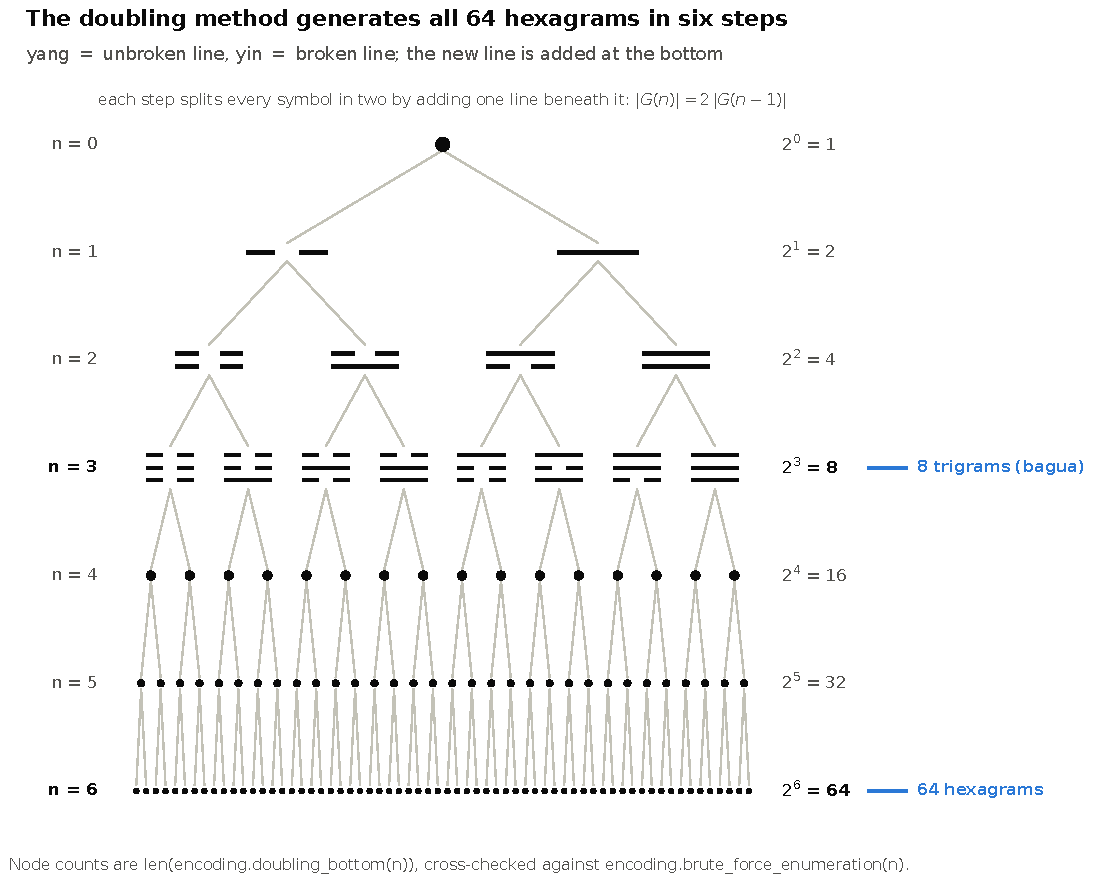
\includegraphics[width=0.85\textwidth]{figures/fig1_doubling.pdf}
\caption{The recursive doubling generation. Each level doubles the number of
symbols, giving the eight trigrams at level three and the sixty-four hexagrams at
level six. The generated set is the same under either convention for placing the
new line.}
\label{fig:doubling}
\end{figure}

\subsection{Algebraic structure}

Theorem~\ref{thm:xor} holds on all $4096$ assignments of the four line states,
with zero mismatches against a line-by-line simulation of the traditional
semantics. Commutativity holds on all $262{,}144$ triples and the involution
property on all $4096$ pairs. For every ordered pair of states there is exactly
one input symbol carrying the first to the second, so the automaton reaches any
state from any other in one input step.

The group identification of Proposition~\ref{prop:group} is confirmed: the
structure is abelian of order $64$ and exponent $2$. Extending to permutations of
line positions, the action of the generated group is faithful and has order
$46{,}080 = 2^6 \cdot 6!$, matching the hyperoctahedral group. This quantity is
not in the received account.

\subsection{Divination probabilities and the failure of independence}

Exact rational evaluation of the three-operation procedure reproduces
Equation~\eqref{eq:linestates} precisely, as rationals rather than as decimal
approximations. A Monte-Carlo simulation of the physical procedure over
$10^{6}$ casts agrees with the exact values to within $2.7 \times 10^{-4}$
(Figure~\ref{fig:linestates}). The marginal change
probability is exactly $1/4$ and the expected number of changing lines is exactly
$3/2$, both matching the received values. The cast hexagram is uniform over the
$64$ states, since each line is yang with probability exactly $1/2$, which
justifies the uniform prior used in the entropy calculation.

\begin{figure}[t]
\centering
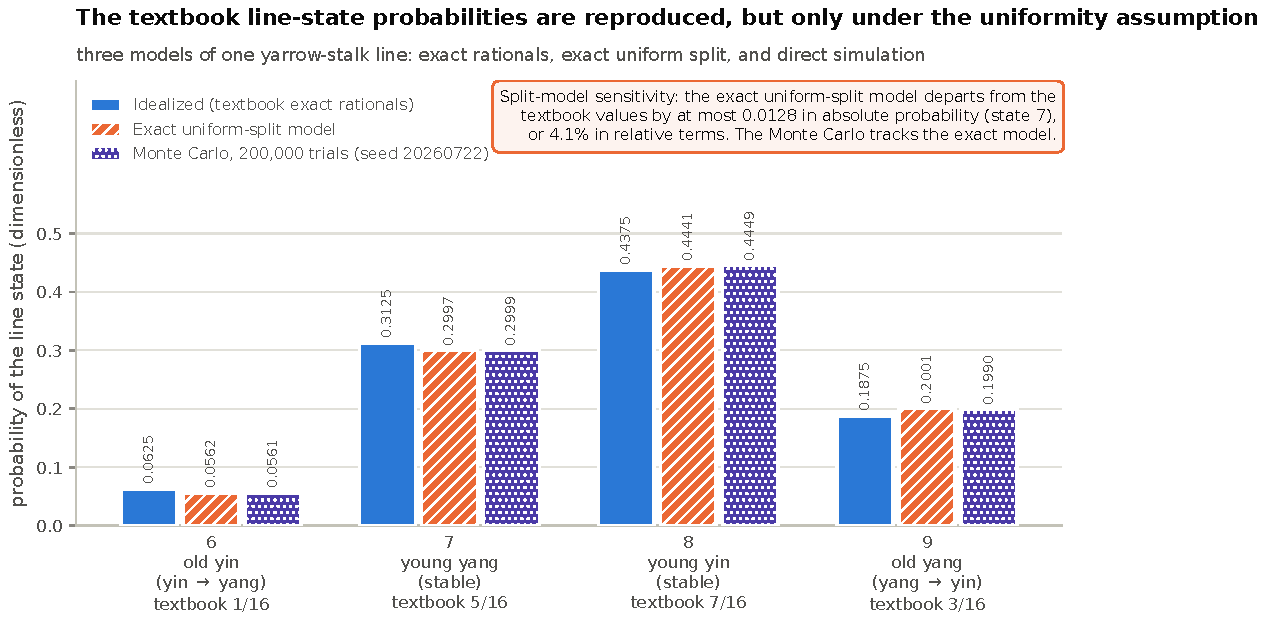
\includegraphics[width=0.85\textwidth]{figures/fig3_line_states.pdf}
\caption{Line-state probabilities under three models. The idealized model
reproduces the received values exactly. The uniform-split model quantifies the
sensitivity of those values to the assumption that the left-heap size is uniform
modulo four. The Monte-Carlo estimate confirms the idealized values.}
\label{fig:linestates}
\end{figure}

The correction is in the conditionals. Equation~\eqref{eq:conditional} gives
$P(\text{change} \mid \text{yang}) = 3/8$ and
$P(\text{change} \mid \text{yin}) = 1/8$. The mutation mask is therefore not
independent of the state. The marginal rate of $1/4$ is a mixture of these two
conditionals weighted by the equal marginals of yang and yin, which is why the
dependence is invisible at the level of the marginal and why the received
analysis could carry an independence assumption without an obvious inconsistency.

The transformed hexagram is yang on any given line with probability $3/8$, not
$1/2$, so it is not uniform.

Under the uniform-split model the four line-state probabilities move by at most
$1.3 \times 10^{-2}$, and the conditionals become $0.400$ and $0.112$. The
idealized values are therefore a good approximation, and the state dependence is
robust to the modelling choice rather than an artifact of it.

\subsection{Stationary behaviour of the two kernels}

The independent-mask kernel of Equation~\eqref{eq:kernelA} is stochastic,
symmetric, irreducible, and aperiodic, and the uniform distribution is exactly
stationary for it. The received Theorem on this point is correct for the kernel
it defines.

The yarrow kernel of Equation~\eqref{eq:kernelB} is stochastic, irreducible, and
aperiodic, but it is not symmetric, and the uniform distribution is not
stationary for it. The product form of Equation~\eqref{eq:stationary} is exactly
stationary, verified in rational arithmetic against the full $64 \times 64$
kernel. It places $729/4096$ of the mass on Kun and $1/4096$ on Qian
(Figure~\ref{fig:stationary}).

\begin{figure}[t]
\centering
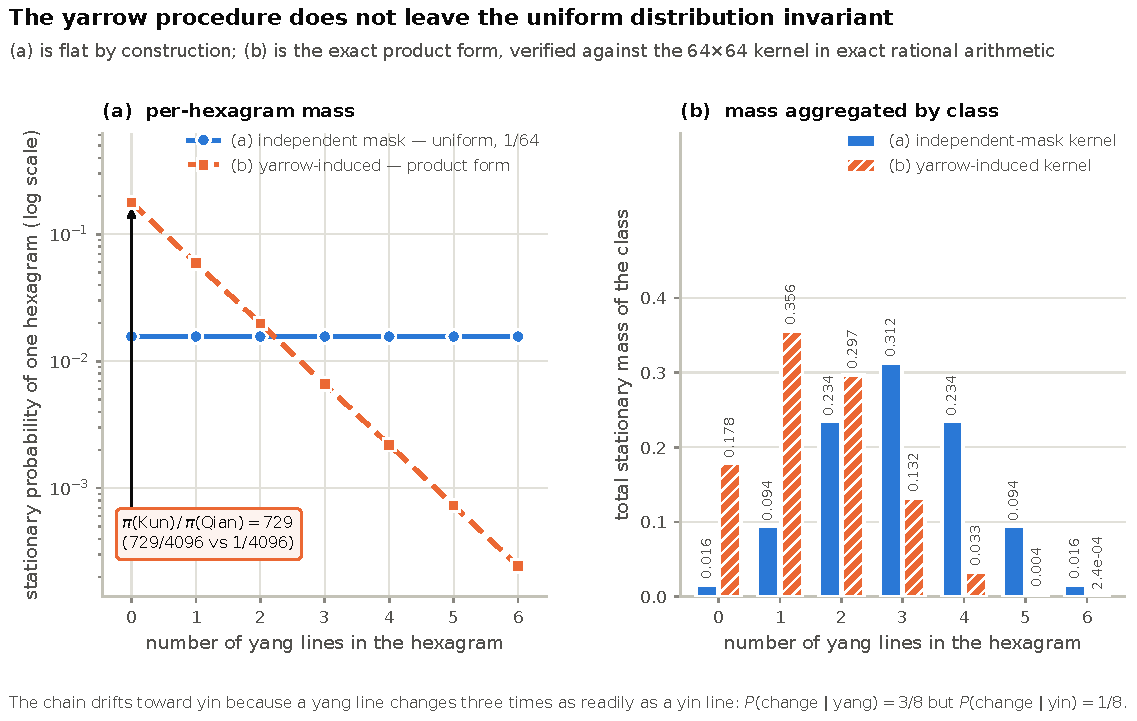
\includegraphics[width=0.85\textwidth]{figures/fig4_stationary.pdf}
\caption{Stationary mass by number of yang lines. The independent-mask kernel is
uniform over the sixty-four states. The kernel induced by the yarrow-stalk
procedure is not, because yang lines change more readily than yin lines. The
ratio between the all-yin and all-yang states is $729$ to $1$.}
\label{fig:stationary}
\end{figure}

Both kernels have spectral gap $1/2$, agreeing with the analytically predicted
eigenvalues $2^{-k}$ with multiplicity $\binom{6}{k}$. Measured worst-case mixing
to total-variation distance $0.01$ takes seven steps for the independent-mask
kernel and eight for the yarrow kernel (Figure~\ref{fig:mixing}). The received
account gives an order-of-magnitude bound of six steps, which the measurement
refines.

\begin{figure}[t]
\centering
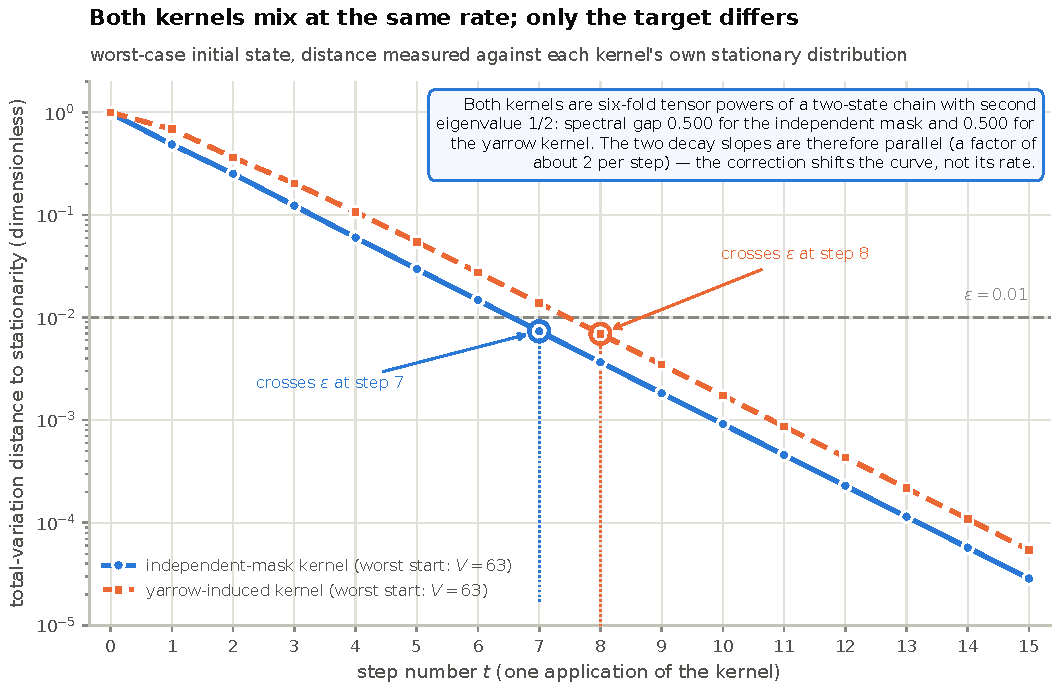
\includegraphics[width=0.85\textwidth]{figures/fig5_mixing.pdf}
\caption{Total-variation distance to stationarity against step number, from the
worst-case start. The two kernels share a spectral gap of $1/2$, so their decay
rates agree even though their stationary distributions do not.}
\label{fig:mixing}
\end{figure}

\subsection{Topology}
\label{sec:topology}

The state-transition graph has $64$ vertices, $192$ edges, and is $6$-regular.
Its diameter is $6$, measured by breadth-first search from all sources, and the
graph distance equals the Hamming distance for every pair. The adjacency spectrum
computed numerically agrees with the analytic prediction of $6-2k$ with
multiplicity $\binom{6}{k}$.

Two quantities require amendment.

The clustering coefficient is exactly zero, not $5/12$. The graph contains no
triangles at all: enumeration over $960$ connected triples returns zero closed
ones. The reason is structural. The graph is bipartite, with the two parts given
by the parity of the number of yang lines and each of size $32$. A bipartite
graph has no odd cycles and therefore no triangles. Equivalently, two neighbours
of a hexagram each differ from it in one line, so they differ from each other in
two lines and are never adjacent. Every clustering coefficient of $\Qsix$ is
zero, and no value in $(0,1]$ can be correct (Figure~\ref{fig:hypercube}).

\begin{figure}[t]
\centering
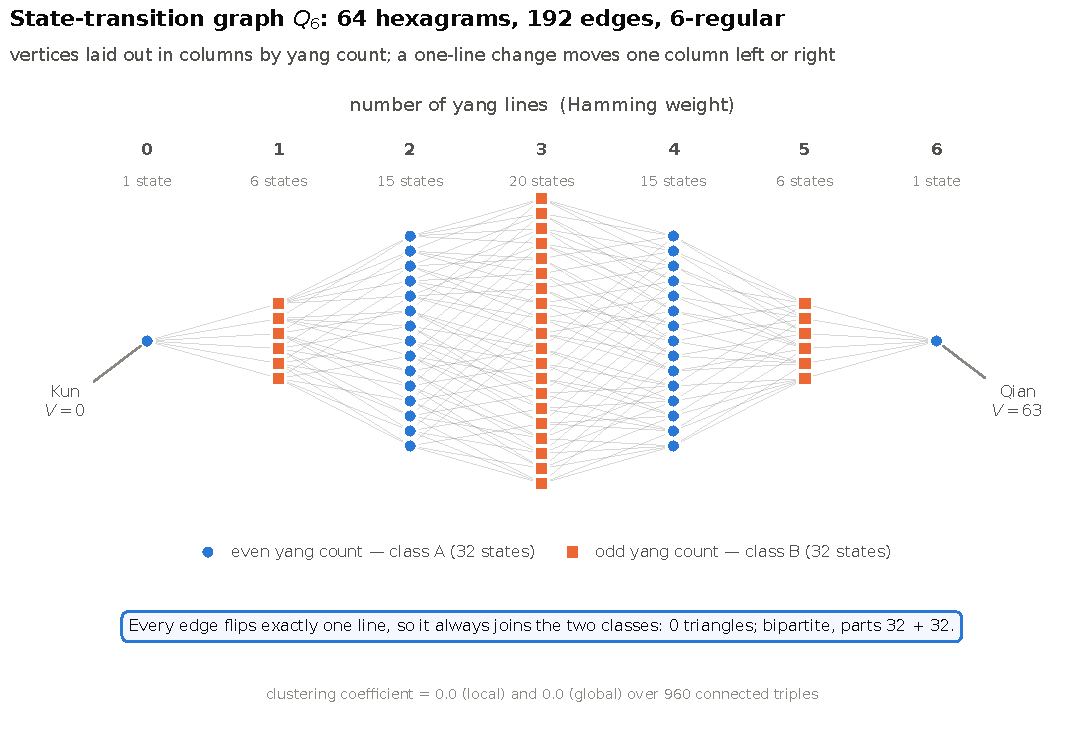
\includegraphics[width=0.9\textwidth]{figures/fig2_hypercube.pdf}
\caption{The state-transition graph, laid out in columns by number of yang lines.
Every edge joins adjacent columns, so the graph is bipartite with parts of size
$32$ and $32$ and contains no triangles. This is why its clustering coefficient
is zero rather than $5/12$.}
\label{fig:hypercube}
\end{figure}

The average shortest-path length is $192/63 \approx 3.048$, not $3$. The value
$3$ is the mean Hamming distance between two independently uniform hexagrams,
which counts the $64$ zero-distance self-pairs. The standard definition of
average shortest-path length excludes them. Both quantities are meaningful and
they are not the same, so we report both.

The Hamming distance distribution between two independent uniform hexagrams has
mean exactly $3$ and variance exactly $3/2$, matching the received values.

\subsection{Information content}

The entropy of a uniformly distributed hexagram is $6$ bits. The entropy of the
independent mutation mask at $p = 1/4$ is $6 H_b(1/4) = 4.8677$ bits, and
Equation~\eqref{eq:miA} gives $I^{A} = 1.1323$ bits. These match the received
values, and the arithmetic of the received calculation is correct for the model
it assumes.

Carrying the state dependence through changes the answer.
Equation~\eqref{eq:miB} evaluated on the joint law of
Equation~\eqref{eq:joint} gives $I^{B} = 1.2326$ bits. The transformation
retains $20.5$ percent of the six bits rather than $18.9$ percent. Relatedly, the
transformed hexagram carries $5.7266$ bits, not $6$, because it is yin-biased
(Figure~\ref{fig:information}).

\begin{figure}[t]
\centering
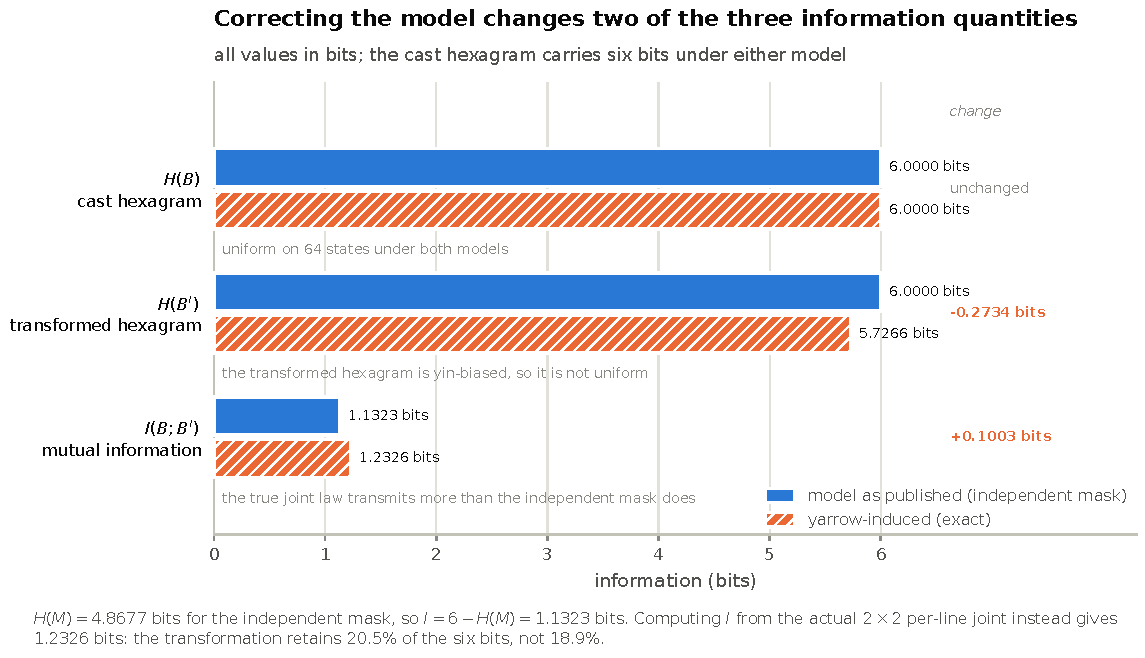
\includegraphics[width=0.85\textwidth]{figures/fig6_information.pdf}
\caption{Information quantities in bits. The cast hexagram carries the full six
bits. The transformed hexagram carries less, because it is yin-biased. The
mutual information between them is higher than the independent-mask model
predicts.}
\label{fig:information}
\end{figure}

\subsection{Orderings}
\label{sec:orderings}

Everything to this point concerns the set of sixty-four hexagrams and the group
acting on it. Neither depends on how the hexagrams are arranged in a sequence.
This section addresses the arrangement, which is where the Earlier Heaven and
King Wen orderings differ, and where the one remaining correction lies.

\paragraph{Two readings of the Earlier Heaven arrangement.}
The classical trigram order is Qian, Dui, Li, Zhen, Xun, Kan, Gen, Kun. Read
with the bottom line as the \emph{most} significant bit, that sequence is $7$
down to $0$, and the sixty-four hexagram sequence extends it from Qian down to
Kun. The arrangement is therefore binary counting, but under the opposite
bit-weight convention from the one adopted in Section~\ref{sec:encoding} for the
algebra. Under the bottom-as-least-significant convention the classical sequence
is a different permutation of the same set, differing at $56$ of the $64$
positions.

This corrects the way the identification is usually stated, including in the
informal version of this analysis. It is worth being precise about what it does
and does not disturb. The two readings are conjugate by the
bit-reversal permutation. A permutation of bit positions is an isometry of the
hypercube, so it preserves every Hamming distance. The two readings consequently
have identical coding profiles, and no distance-based property of the
arrangement can depend on the choice. What the choice does fix is the direction
of the enumeration, and that is exactly the question
of~\cite{maitre2023fuxi}. Our contribution here is to make the dependence exact:
the set is convention-independent, the sequence is not, and the two candidate
sequences are related by bit reversal.

\paragraph{The Earlier Heaven arrangement is not an optimal code.}
Under either reading, the arrangement changes $120$ lines across its $63$ steps,
a mean of $1.905$ lines per step, and only $32$ of the $63$ steps change a single
line. A reflected binary (Gray) code on the same sixty-four states changes one
line at every step, for a total of $63$ and a mean of $1.000$. Binary counting is
not a Gray code. Any claim that the arrangement minimizes change from one
hexagram to the next is therefore false, and the optimum it is sometimes said to
achieve is achieved by a different ordering.

\paragraph{The King Wen couplet structure.}
Tradition holds that the King Wen sequence consists of thirty-two couplets, in
which the second hexagram is the first turned upside down, except where a
hexagram is unchanged by inversion, in which case the couplet is completed by
the complement instead.

The claim is well posed before any sequence data is consulted. Assign every
hexagram its reversal, or its complement when it is its own reversal. That
assignment is a perfect matching on the sixty-four states. The complement of a
palindromic hexagram is itself palindromic, so the eight palindromes close among
themselves into four pairs, leaving twenty-eight reversal pairs.

The claim holds exactly. All thirty-two couplets of the King Wen sequence are
accounted for, twenty-eight by reversal and four by complement, with none
unexplained. The four complement couplets are King Wen $1$--$2$, $27$--$28$,
$29$--$30$ and $61$--$62$, which are precisely the couplets whose members are
their own reversal.

Its improbability can be counted rather than estimated. If the claim holds, the
sequence lists thirty-two matched pairs consecutively, so the favourable
permutations number $32! \cdot 2^{32}$ out of $64!$, a probability of
$8.9 \times 10^{-45}$. A random ordering satisfies fewer than one couplet on
average. No simulation can reach this magnitude, which is why the value is
computed exactly.

\paragraph{The two criteria come apart.}
The King Wen sequence satisfies the symmetry criterion perfectly and does not
satisfy the distance criterion at all. Its mean consecutive Hamming distance is
$3.349$, against a random null of $3.044 \pm 0.152$ over four thousand random
orderings. It therefore sits about two standard deviations \emph{above} random
rather than below it. Only $2$ of its $63$ steps change a single line
(Figure~\ref{fig:orderings}).

The two criteria are independent, and the sequence optimizes one of them. That
is a fact about the sequence, not an inference about intent, and we draw no
conclusion about why it was built the way it was.

\begin{figure}[t]
\centering
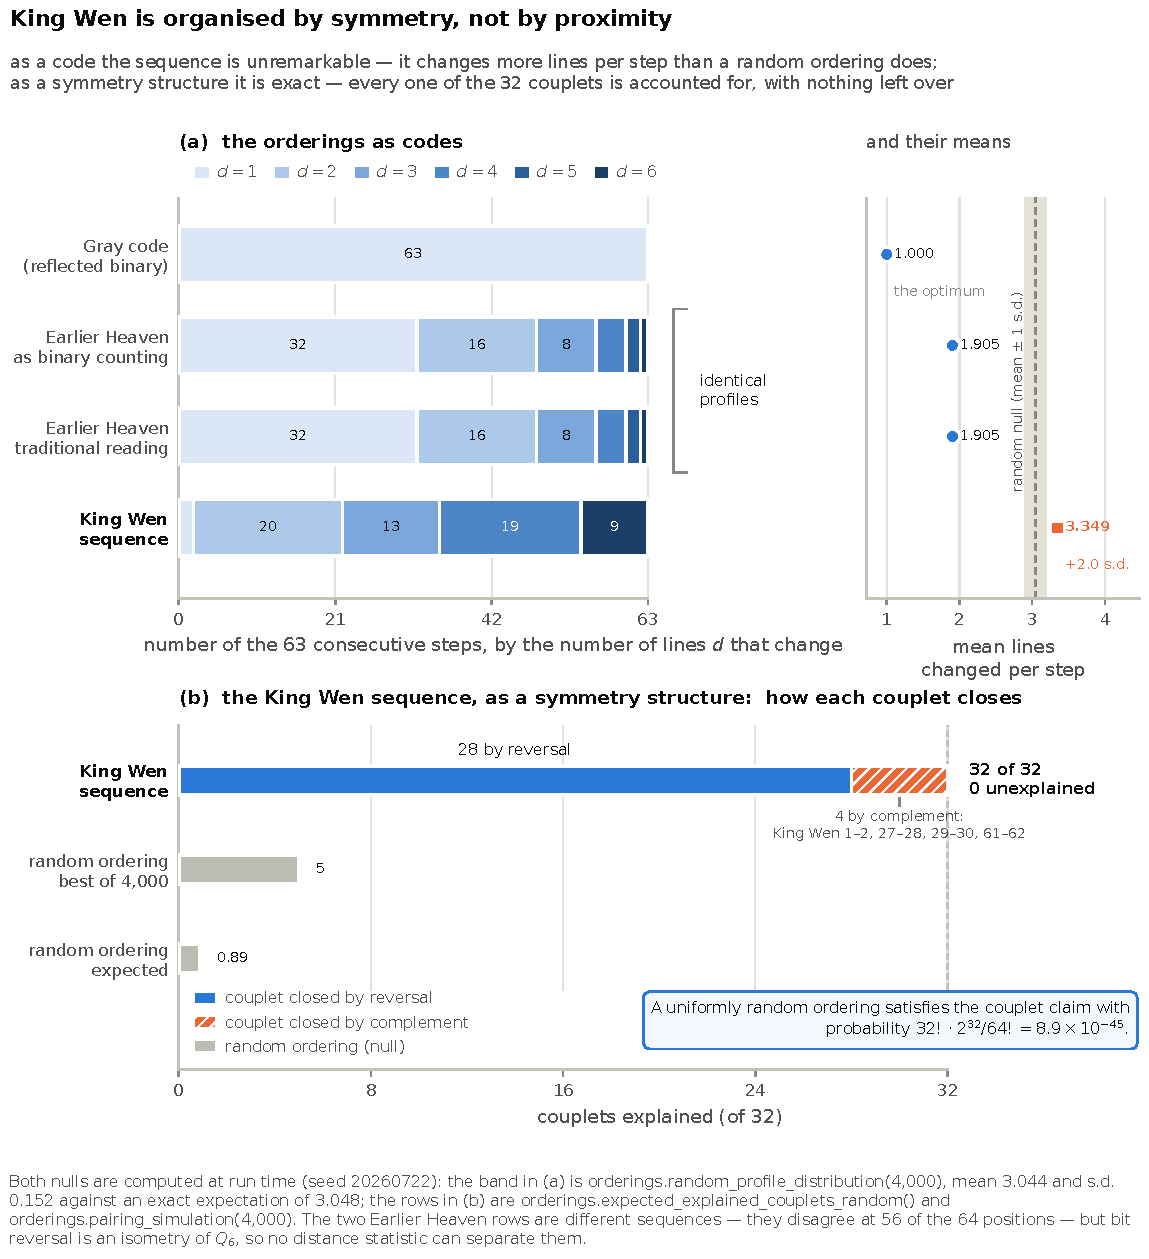
\includegraphics[width=0.92\textwidth]{figures/fig7_orderings.pdf}
\caption{Four orderings of the same sixty-four hexagrams, compared as codes. The
Gray code is optimal. The Earlier Heaven arrangement is binary counting under
either reading, and the two readings have identical profiles because bit
reversal is an isometry. The King Wen sequence sits slightly above the random
null, while satisfying a symmetry criterion that a random ordering meets with
probability $8.9 \times 10^{-45}$.}
\label{fig:orderings}
\end{figure}

\subsection{The genetic-code dimension count}
\label{sec:genetic}

Each nucleotide is commonly described by three binary dichotomies: purine against
pyrimidine, amino against keto, and strong against weak. Applying three
dichotomies at three codon positions suggests nine binary degrees of freedom,
which would give $2^9 = 512$ codons rather than $64$.

Gaussian elimination over $\mathrm{GF}(2)$ on the $4 \times 3$ dichotomy matrix
returns rank $2$, not $3$. The dependency is exact and checkable by hand: for all
four nucleotides, the strong/weak bit is the exclusive-or of the
purine/pyrimidine bit and the amino/keto bit. Writing the three bits in that
order, adenine is $(1,1,0)$, cytosine is $(0,1,1)$, guanine is $(1,0,1)$, and
uracil is $(0,0,0)$, and in each case the third coordinate is the sum of the
first two modulo two.

Each nucleotide therefore carries two free bits, not three, and a codon carries
six, which gives $2^6 = 64$. The corrected count reaches the same number by a
route that is arithmetically consistent. We confirm separately that the resulting
two-bit encoding is injective on the four nucleotides and that the induced map
from the $64$ codons onto $\{0,\dots,63\}$ is a bijection.

We note what this does and does not establish. It establishes that both sets have
$64$ elements and that a bijection exists. A bijection between two sets of the
same finite size always exists, so the bijection alone carries no information
about any relationship between the two systems.

\subsection{Robustness}

Three stress tests bound the results. First, the exact and idealized yarrow
models are compared, and the state dependence that drives the main correction
survives under both. Second, the analytic and numerical spectra are computed by
independent routes and compared for both kernels and for the adjacency matrix.
Third, quantities that are rational are compared exactly rather than within a
tolerance, which removes floating-point accumulation as a source of agreement.
The Monte-Carlo checks are the only sampled results, and they are reported with
their trial count, seed, and observed deviation.

\section{Discussion}

\subsection{What the corrections change}

The corrections divide into three kinds, and they do not all have the same
weight.

The clustering coefficient and the genetic-code dimension count are local
errors. They do not propagate. Correcting the clustering coefficient to zero
replaces a number with a structural fact, namely that the state graph is
bipartite, which is more informative than the number it replaces. Correcting the
dimension count removes an inconsistency while leaving the count of $64$ intact.

The bit-weight convention is a different kind again. It is not a wrong number but
a wrong attribution: the arrangement is binary counting, and the reading under
which that is true was misidentified. Nothing downstream moves, because the two
readings differ by an isometry. What changes is the precision with which the
identification can be stated, and that is the question the historical literature
has actually been arguing about. We note that this is the one correction we
introduced ourselves, in the informal version of this analysis, and that it was
caught by the same procedure as the others.

The independence failure is different, because it propagates. It changes the
stationary distribution from uniform to a product form with a $729$-fold spread,
it changes the mutual information, and it changes the entropy of the transformed
hexagram. The reason it went unnoticed is instructive. The marginal change rate
is exactly $1/4$, which is what the received analysis checked, and the cast
hexagram is exactly uniform, which is what the entropy calculation needed. Both
of those are true. The independence assumption is a third claim that neither of
them implies, and it is false.

The substantive consequence is that the system has a direction. Under the
kernel the divination procedure induces, repeated transformation is not a
symmetric random walk on the hypercube. It is a biased walk with a preferred
region, and the bias points toward yin. Whether that asymmetry is a designed
feature of the procedure or an incidental consequence of the counting rules is
not something the formalization can settle, and we do not claim it is.

\subsection{Rival explanations}

Three alternative readings deserve to be addressed before any of this is
generalized.

The first is that the results are artifacts of the encoding. This is partly
true and we have tried to bound it. The graph invariants are invariant under
relabelling, so the clustering result does not depend on the encoding at all.
The stationary distribution is stated in terms of the number of yang lines
rather than in terms of bit values, so it is also encoding-independent. The
enumeration order is the one quantity that genuinely depends on convention, and
we therefore report it under both conventions rather than picking one.

The second is that the yarrow-stalk procedure has attested variants, and the
probabilities depend on which variant is modelled. This is correct. We model the
three-operation procedure on $49$ stalks under two explicit assumptions about how
the pile is divided, and we report both. The coin-based method in common use has
a different distribution over line states and would give different numbers. Our
claim is about the procedure we model, not about divination in general.

The third is that the ordering of the arrangement admits more than one defensible
reconstruction. This is correct, and it is the one place where a convention
genuinely changes an answer, as Section~\ref{sec:orderings} shows. We handle it
in two ways. The algebraic, topological, and probabilistic results do not rely on
any ordering at all, being properties of the set and its structure. Where an
ordering is unavoidable, we report both readings and show they are conjugate by
bit reversal, which is an isometry, so no distance-based conclusion can depend on
the choice. The couplet result for the King Wen sequence is likewise invariant,
since reversal and complementation are defined on hexagrams rather than on
positions.

\subsection{Relation to discrete computational models, and the limits of that
relation}
\label{sec:scope}

The system has features that recur in discrete models of physics. Its state space
is finite, its transition rules are local in the sense that each generator
affects one line, its states are generated recursively by bifurcation, and its
deterministic dynamics are information preserving because exclusive-or is an
involution. These are the features that motivate the broader literature on
computable and discrete universe models, which represents dynamics as rewriting
rules on discrete structures~\cite{wolfram2002new,gorard2020relativistic},
as quantum computation~\cite{lloyd2005computational}, or as causal
sets~\cite{sorkin2005causal}, and which has been surveyed by
Zenil~\cite{zenil2012introducing}.

We think the honest statement of the relation is a negative one, and we want to
be specific about why.

The shared features listed above are shared by every system built from iterated
binary splitting. They are consequences of the construction, not evidence of a
common origin. A finite state space with local involutive generators is what one
gets by definition when one takes a finite abelian group of exponent two and its
Cayley graph. Finding that structure in the hexagram arrangement is finding that
the arrangement was built by repeated bifurcation, which is what the doubling
generation says it was built by. Nothing further follows.

The scale gap is the second reason. The formalized system has $64$ states. Any
comparison to a physical theory is a comparison across many orders of magnitude,
and the analogy does no work at that distance. Our system is a useful object
precisely because it is small enough to enumerate exhaustively, which is the
property that let us find the errors reported here. It is not small in a way that
makes it a scale model of anything larger.

We therefore make no claim that the arrangement anticipated binary computation,
the genetic code, or any model of discrete physics. The recurrence of powers of
two across unrelated systems is what binary splitting produces, and it is not
evidence of a relationship. The bijection between hexagrams and codons verified
in Section~\ref{sec:genetic} is a statement about two sets of size $64$; a
bijection between finite sets of equal size always exists, so its existence
carries no information.

Predictions in this area, such as the error-minimizing structure of the genetic
code~\cite{freeland1998genetic} or observable signatures of discrete
spacetime~\cite{mattingly2005modern}, are predictions of those independent
hypotheses. They are not predictions of the present formalization, and we do not
present them as such. Nor is the simulation argument~\cite{bostrom2003simulation}
engaged by anything here; it is a probabilistic argument about posthuman
computation, and a formal model of a symbolic system neither supports nor
undermines it.

We also make no claim about the divinatory or interpretive tradition. The
probability model describes the procedure by which line states are produced. It
says nothing about what those line states are taken to mean.

\subsection{Limitations}

The formalization covers the Earlier Heaven arrangement, the King Wen sequence,
and the three-operation yarrow procedure. It does not cover the coin method, the
line-position correspondences used in traditional interpretation, or any of the
commentarial apparatus.

The King Wen results depend on sequence data, which is the one place this work
relies on an external source rather than on construction. We reconciled four
independent sources and checked every entry against anchors derived from the
trigram composition, and the table passes eight structural checks. One source
proved to contain a genuine error, which the checks caught. We note the
dependence because it is different in kind from the rest of the paper.

The probability results depend on a model of how the pile is divided. We report
two such models and show the main conclusion is stable across them, but neither
model is derived from empirical observation of how people actually divide a pile
of stalks, and we are not aware of data that would settle it.

The Monte-Carlo results are estimates. They are reported with trial counts and
seeds, and they agree with the exact computations, but they are not independent
evidence for those computations since they simulate the same model.

Finally, a note on the citations. The twenty-two references circulating with the
informal version of this analysis were each checked against a publisher record,
a DOI, or an authoritative index. Nine were correct, twelve carried at least one
wrong field, and one did not exist: an article attributed to \emph{Studies of
Zhouyi} 2006(3): 62--67 is absent from that issue's table of contents, and the
description appears to belong to a different article in a different journal,
which we cite instead~\cite{sun2018dayan}. The audit is recorded in the
repository. Two of the comparative genetic-code references sit in venues from
publishers widely listed as predatory, which we note so that readers can weigh
them accordingly.

\section{Conclusion}

We have given a computational formalization of the Fuxi Earlier Heaven hexagram
system and machine-checked the quantitative claims that the received account
makes about it. The changing-line mechanism is bitwise exclusive-or, verified on
all $4096$ line-state assignments, and the transition structure is the
elementary abelian group $\Ztwo^6$ whose Cayley graph is the six-dimensional
hypercube. Twenty-five of forty-seven checked claims are confirmed and five are
refined. Among the confirmed is a structural claim about the King Wen sequence:
its thirty-two couplets are related by inversion, or by complementation for the
eight hexagrams that are their own inversion, and a random ordering reproduces
that structure with probability $8.9 \times 10^{-45}$. The same sequence is not
optimized as a code, which separates the two criteria under which an arrangement
might be called ordered.

Eight are corrected. The state-transition graph is bipartite and therefore has a
clustering coefficient of exactly zero rather than $5/12$. The genetic-code
dichotomies are dependent over $\mathrm{GF}(2)$, giving two free bits per
nucleotide rather than three. The Earlier Heaven arrangement is binary counting
only when the bottom line is read as the most significant bit, the opposite of
the convention that makes the algebra convenient, and the two readings differ at
$56$ of $64$ positions while sharing every distance-based property. Most
consequentially, the yarrow-stalk procedure
makes a yang line change three times as often as a yin line, so the mutation mask
is not independent of the state. The kernel the procedure induces is asymmetric,
its stationary distribution is the product form
$\pi(h) \propto (3/4)^{6-y(h)}(1/4)^{y(h)}$ rather than uniform, and the mutual
information between the cast and transformed hexagram is $1.233$ bits rather than
$1.132$.

The scope of these results is the formal model. They establish properties of a
six-bit state machine and of a probability model of one divination procedure.
They do not establish anything about the interpretive tradition, and they do not
support comparisons between this system and physical theory beyond the
observation that both can be built by iterated binary splitting.

The methodological point generalizes further than the specific corrections do.
Four distinct errors persisted in an account of a $64$-state system, which is
small enough to enumerate completely on any computer. One of them we introduced
ourselves and caught only by running the arrangement rather than describing it.
They persisted because the account was written rather than executed.
Formalizations of historical symbolic systems are worth executing, and the cost
of doing so is low.

The same discipline applied to the bibliography found a comparable rate. That
suggests the problem is not specific to this subject matter.

\section*{Code and data availability}

The verification suite, the figure scripts, and the source of this manuscript are
available at \url{https://github.com/AwareLiquid/The-Fuxi-Binary-System-Math}. All
results in this paper are regenerated by running \texttt{python verify\_all.py}
from the \texttt{code} directory. The suite requires only the Python standard
library; NumPy is used solely for the numerical spectra that cross-check the
analytic ones.

\begin{thebibliography}{99}

\bibitem{aiton1981gorai}
Aiton E J, Shimao E.
Gorai Kinz\=o's study of Leibniz and the I ching hexagrams.
\emph{Annals of Science}, 1981, 38(1): 71--92.
\href{https://doi.org/10.1080/00033798100200121}{doi:10.1080/00033798100200121}.

\bibitem{maitre2023fuxi}
Maitre M-J.
Is the \emph{Fuxi liushisi gua fangwei} diagram attributed to Shao Yong binary?
Clarifying a consequence of its analogy with the binary arithmetic of Leibniz.
\emph{Science in Context}, 2023, 36(1): 38--59.
\href{https://doi.org/10.1017/S0269889725100665}{doi:10.1017/S0269889725100665}.
Published online 15 August 2025.

\bibitem{goldenberg1975algebra}
Goldenberg D S.
The algebra of the I Ching and its philosophical implications.
\emph{Journal of Chinese Philosophy}, 1975, 2(2): 149--179.
\href{https://doi.org/10.1111/j.1540-6253.1975.tb00366.x}{doi:10.1111/j.1540-6253.1975.tb00366.x}.

\bibitem{hayata2012coding}
Hayata K.
A coding-theoretical approach to analyzing sequential patterns of the sixty-four
hexagrams in the I Ching.
\emph{Forma}, 2012, 27(1): 55--65.

\bibitem{schoter1998boolean}
Sch\"oter A.
Boolean algebra and the Yi Jing.
\emph{The Oracle: The Journal of Yijing Studies}, 1998, 2(7): 19--34.

\bibitem{schoter2008bipolar}
Sch\"oter A.
Bipolar change.
\emph{Journal of Chinese Philosophy}, 2008, 35(2): 297--317.
\href{https://doi.org/10.1111/j.1540-6253.2008.00479.x}{doi:10.1111/j.1540-6253.2008.00479.x}.

\bibitem{hu2017iching}
Hu Z, Petoukhov S V, Petukhova E S.
I-Ching, dyadic groups of binary numbers and the geno-logic coding in living
bodies.
\emph{Progress in Biophysics and Molecular Biology}, 2017, 131: 354--368.
\href{https://doi.org/10.1016/j.pbiomolbio.2017.08.018}{doi:10.1016/j.pbiomolbio.2017.08.018}.

\bibitem{castrochavez2012defragged}
Castro-Ch\'avez F.
Defragged binary I Ching genetic code chromosomes compared to Nirenberg's and
transformed into rotating 2D circles and squares and into a 3D 100\% symmetrical
tetrahedron coupled to a functional one to discern start from non-start
methionines through a stella octangula.
\emph{Journal of Proteome Science and Computational Biology}, 2012, 1(1): 3.
\href{https://doi.org/10.7243/2050-2273-1-3}{doi:10.7243/2050-2273-1-3}.

\bibitem{lien1997physicochemical}
Lien E J, Das A, Nandy P, Ren S.
Physicochemical basis of the universal genetic codes: quantitative analysis.
\emph{Progress in Drug Research}, vol.~48. Birkh\"auser Basel, 1997: 9--25.
\href{https://doi.org/10.1007/978-3-0348-8861-5_1}{doi:10.1007/978-3-0348-8861-5\_1}.

\bibitem{sun2018dayan}
Sun D.
Analysis of the Dayan divination method and the yarrow-divination probabilities
of the Yi hexagrams.
\emph{Literature, History and Philosophy}, 2018(1): 47--59. In Chinese.

\bibitem{tang2017monte}
Tang Y.
Monte Carlo simulation of the sixty-four hexagrams of the I Ching.
\emph{The Northern Forum}, 2017(5): 43--46. In Chinese.

\bibitem{freeland1998genetic}
Freeland S J, Hurst L D.
The genetic code is one in a million.
\emph{Journal of Molecular Evolution}, 1998, 47(3): 238--248.
\href{https://doi.org/10.1007/PL00006381}{doi:10.1007/PL00006381}.

\bibitem{wolfram2002new}
Wolfram S.
\emph{A New Kind of Science}.
Champaign, IL: Wolfram Media, 2002. ISBN 1-57955-008-8.

\bibitem{gorard2020relativistic}
Gorard J.
Some relativistic and gravitational properties of the Wolfram model.
arXiv:2004.14810, 2020.
Published as \emph{Complex Systems}, 2020, 29(2): 599--654.

\bibitem{lloyd2005computational}
Lloyd S.
The computational universe: quantum gravity from quantum computation.
arXiv:quant-ph/0501135v1, 2005.

\bibitem{sorkin2005causal}
Sorkin R D.
Causal sets: discrete gravity.
In: Gomberoff A, Marolf D, eds. \emph{Lectures on Quantum Gravity}.
New York: Springer, 2005: 305--327.
\href{https://doi.org/10.1007/0-387-24992-3_7}{doi:10.1007/0-387-24992-3\_7}.

\bibitem{zenil2012introducing}
Zenil H.
Introducing the computable universe.
In: Zenil H, ed. \emph{A Computable Universe: Understanding and Exploring Nature
as Computation}. World Scientific, 2012: 1--20.
\href{https://doi.org/10.1142/9789814374309_0001}{doi:10.1142/9789814374309\_0001}.

\bibitem{mattingly2005modern}
Mattingly D.
Modern tests of Lorentz invariance.
\emph{Living Reviews in Relativity}, 2005, 8(1): 5.
\href{https://doi.org/10.12942/lrr-2005-5}{doi:10.12942/lrr-2005-5}.

\bibitem{bostrom2003simulation}
Bostrom N.
Are you living in a computer simulation?
\emph{The Philosophical Quarterly}, 2003, 53(211): 243--255.
\href{https://doi.org/10.1111/1467-9213.00309}{doi:10.1111/1467-9213.00309}.

\end{thebibliography}

\end{document}
